% vim: spell spl=pt fo+=tcwa tw=98 nonu fdc=0
% vim: ts=4 sw=4 sts=4 expandtab
\documentclass{beamer}
\usepackage[brazil]{babel}
\usepackage[utf8]{inputenc}
\usepackage[T1]{fontenc}
\usepackage{graphicx,epstopdf,wrapfig,caption,url}
\usepackage{mathtools}
\usepackage{multirow}

\title[MIHS]{Media Independent Handover Services}
\author{Higor Eurípedes P. F. A.}
\institute[IFTO]{Instituto Federal de Educação, Ciência e Tecnologia do Tocantins}
\date[Fevereiro 2012]{28 de fevereiro de 2012}

\AtBeginSection[]
{
  \begin{frame}
    \frametitle{Media Independent Handover Services}
    \tableofcontents[currentsection,currentsubsection]
  \end{frame}
}
\AtBeginSubsection[]
{
  \begin{frame}
    \frametitle{Media Independent Handover Services}
    \tableofcontents[currentsection,currentsubsection]
  \end{frame}
}

\usetheme{default}
\usecolortheme{seahorse}

\begin{document}
    \frame{\titlepage}

    \frame{
        \frametitle{Apresentação}
        \tableofcontents
    }


    \section{O padrão IEEE 802.21}

    \frame{
        \frametitle{\insertsectionhead}

        \begin{block}{}
            \begin{itemize}

                \item Facilitador de transições entre redes heterogêneas.
                \item Abstração das camadas de enlace e rede (MIHF).
                \item Interface unificada inter-tecnologia. 

            \end{itemize} 

        \end{block}
    }
    
    \frame{
        \frametitle{\insertsectionhead}

        \begin{figure}
            \includegraphics[width=\textwidth]{apresentacao-fev-2012/visaogeral.eps}
        \end{figure}
    }

    \subsection{A Media Independent Handover Function (MIHF)}

    \frame{
        \frametitle{\insertsubsectionhead}
       
        \begin{columns}[c]
        \column{.7\textwidth}

        \begin{block}{O que é e o que faz?}
            \begin{itemize}

                \item É uma entidade lógica posicionada camadas 2 e 3.
                \item Abstrai camadas inferiores por meio de serviços:

                \begin{itemize}

                    \item Media Independent Information Service.
                    \item Media Independent Event Service.
                    \item Media Independent Command Service.

                \end{itemize}

                \item Pode se comunicar com outras MIHF.

            \end{itemize}

        \end{block}

        \column{.3\textwidth}
        \begin{figure}
            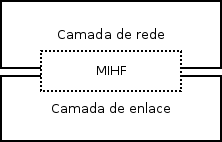
\includegraphics[width=\textwidth]{apresentacao-fev-2012/posicionamento.eps}
        \end{figure}
        \begin{figure}
            \includegraphics[width=\textwidth]{apresentacao-fev-2012/servicos.eps}
        \end{figure}
        \end{columns}
    }

    \frame{
        \frametitle{\insertsubsectionhead}

        \begin{block}{Procedimento simplificado de \textit{handover}}

            \begin{figure}
                \includegraphics[width=\textwidth]{apresentacao-fev-2012/handoversimplificado.eps}
            \end{figure}

        \end{block}
    }

    \section{Modelo de R. Tawil, G. Pujolle e J. Demerjian}
    
    \frame{
        \frametitle{\insertsectionhead}
        %\framesubtitle{Media Independent Command Service (MICS)}


        \begin{itemize}

            \item Decisão distribuida de handover vertical.

            \item \textit{Network Quality Value}.
                \[
                    NVQ_i = \sum_{i=1,j=1}^{N,n_p^+}W_j * P_{ij} + \sum_{i=1,k=1}^{N,n_{p'}^-}W_k 
                    * \frac{1}{P'_{ik}}
                \]


% NVQi representa a qualidade da i-ésima rede. Pij representa os parametros benéficos (largura de 
% banda, segurança etc) enquanto P'ik representa os parametros maléficos (custo, consumo de 
% energia). Wj e Wk são os pesos dados pelo usuário a cada parametro Pij e P'ik, respectivamente.  
% N é o número de redes e np+ e np'- são o numero de parametros benéficos e maléficos, 
% respectivamente.
%somatório de Wj * Pij em que i varia de 1 até n e j varia de 1 até np+

            \item Primitivas reduzidas.
                \begin{table}[h!]
                    \resizebox{\textwidth}{!}{
                        \begin{tabular}[b]{ l | l | l | l }
                            Primitiva & Serviço & Padrão & Descrição \\
                            \hline
                            MIH\_Link\_Going\_Down   & MIES & Sim & O link poderá cair em breve. \\
                             MIH\_Handover\_Initiate & MICS & Não & Inicia o handover. \\
                            MIH\_Get\_Status         & MICS & Não & Retorna o estado do link. \\
                            MIH\_Switch              & MICS & Não & Efetua a troca entre links. \\
                            MIH\_Get\_Information    & MIIS & Não & Solicita informações ao                       
                            repositório.\\
                            \hline
                        \end{tabular}
                    }
                \end{table}
        \end{itemize}
    }
    \frame{
        \frametitle{\insertsectionhead}

        \begin{figure}
            \includegraphics[scale=.25]{apresentacao-fev-2012/esquema-dvhd.eps}
        \end{figure}
    }
    
    \frame{
        \frametitle{\insertsectionhead}

        \begin{figure}
            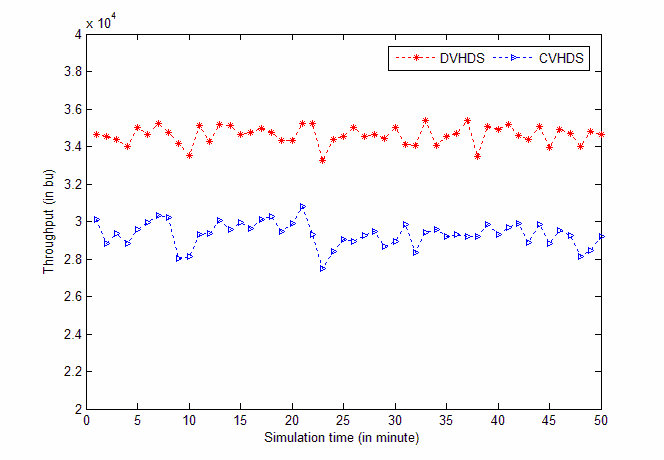
\includegraphics[width=\textwidth]{apresentacao-fev-2012/dvhds-throughput.png}
        \end{figure}
    }

    \frame{
        \frametitle{\insertsectionhead}

        \begin{figure}
            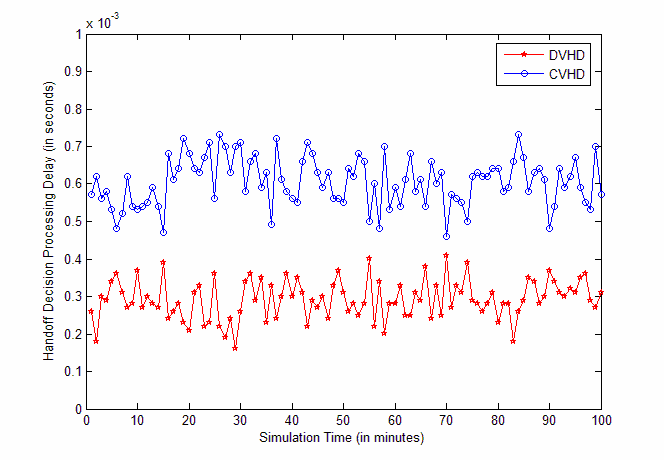
\includegraphics[width=\textwidth]{apresentacao-fev-2012/dvhds-procdelay.png}
        \end{figure}
    }

    \section{Estudo de P. Machań, S. Serwin e J Woźniak}
    
    \frame{
        \frametitle{\insertsectionhead}
    
        \begin{itemize}

            \item Compara performance entre ambientes com e sem suporte a \textit{soft-handover}.

            \item Resultados: ideal pra aplicações multimídia e atraso 8\% menor.
            
            \begin{table}[ht]

                \caption{Pacotes perdidos}

                \begin{tabular}{ l | l | l }
                    \textbf{Carga (Kbps)} & \textbf{hard-handover} & \textbf{soft-handover} \\
                    \hline
                    100 & 450 & 0 \\
                    200 & 835 & 0 \\
                    384 & 1650 & 2 \\
                    400 & 15734 & 29419\\
                    \hline
                \end{tabular}
                
            \end{table}

        \end{itemize}
    }
    
    \frame{
        \frametitle{\insertsectionhead}
        \begin{figure}[ht]
            \includegraphics[width=\textwidth]{apresentacao-fev-2012/machan.eps}
            \caption{Tempo de handover em relação à carga de rede.}
        \end{figure}
    }

    \section{Proposta}

    \frame{
        \frametitle{\insertsectionhead}
        \begin{block}{}

            \begin{itemize}

                \item 3G e 802.11.
                \item MIHFs cliente e servidor.
                \item Primitivas:
                    \begin{table}[h!]
                        \resizebox{\textwidth}{!}{
                            \begin{tabular}[b]{ l | l | l }
                                Primitiva & Serviço & Descrição \\
                                \hline
                                MIH\_Link\_Up          & MIES & O link está disponível. \\
                                MIH\_Link\_Down        & MIES & O link está indisponível. \\
                                MIH\_Link\_Going\_Down & MIES & O link poderá cair em breve. \\
                                MIH\_Link\_Switch      & MICS & Realiza o \textit{handover}. \\
                                 MIH\_Report           & MICS & Obtém informações sobre uma estação. \\
                                      MIH\_Discovery   & MIIS & Procura MIHFs servidoras na rede.  \\
                                \hline
                            \end{tabular}
                        }
                    \end{table}
            \end{itemize}
        \end{block}
    }
    
    \frame{
        \frametitle{\insertsectionhead}
        \begin{figure}[ht]
            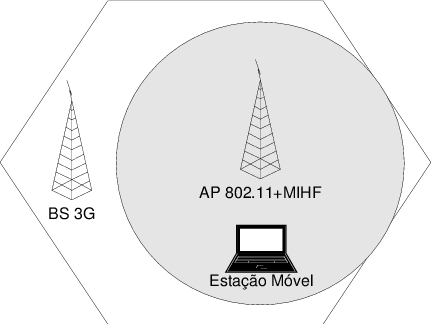
\includegraphics[scale=.5]{apresentacao-fev-2012/ambiente.eps}
            \caption{Cenário proposto.}
        \end{figure}
    }

    \frame{
        \frametitle{\insertsectionhead}
        \begin{figure}[ht]
            \includegraphics[width=\textwidth]{apresentacao-fev-2012/soft-handover.eps}
            \caption{Processo de \textit{soft-handover} no modelo proposto.}
        \end{figure}
    }

\end{document}

